\documentclass[12pt]{article}
\usepackage[UTF8]{ctex}
\usepackage{amsmath, amssymb, amsthm}
\usepackage{graphicx}
\usepackage{tikz}
\usepackage{pgfplots} % 使用 pgfplots 绘制函数图像,便于控制尺寸
\pgfplotsset{compat=1.18} % 设置 pgfplots 兼容性版本
\usepackage{geometry}
\usepackage{hyperref}
\usepackage[svgnames]{xcolor}
\usepackage{fancyhdr}

\geometry{a4paper, left=2cm, right=2cm, top=2.5cm, bottom=2.5cm}

% --- 定理环境设置 ---
\newtheoremstyle{mytheoremstyle}
  {\topsep} % Space above
  {\topsep} % Space below
  {\itshape} % Body font
  {} % Indent amount
  {\bfseries\color{RoyalBlue}} % Theorem head font
  {.} % Punctuation after theorem head
  {.5em} % Space after theorem head
  {} % Theorem head spec (can be left empty, meaning `normal')
\theoremstyle{mytheoremstyle}
\newtheorem{theorem}{不等式}

% --- 颜色定义 ---
\definecolor{MyBlue}{RGB}{0, 80, 150}
\definecolor{MyGreen}{RGB}{0, 150, 80}
\definecolor{MyRed}{RGB}{192, 0, 0}
\definecolor{MyPurple}{RGB}{102, 0, 204}
\definecolor{MyGray}{RGB}{100, 100, 100}


% --- 超链接设置 ---
\hypersetup{
    colorlinks=true,
    linkcolor=MyBlue,
    filecolor=magenta,      
    urlcolor=cyan,
}

% --- 页面样式 ---
\pagestyle{fancy}
\fancyhf{}
\fancyhead[C]{\textcolor{MyGray}{\leftmark}}
\fancyfoot[C]{\textcolor{MyGray}{\thepage}}
\renewcommand{\headrulewidth}{0.4pt}
\renewcommand{\footrulewidth}{0.4pt}

% --- 命令定义 ---
\newcommand{\dd}{\mathrm{d}}

\title{\textcolor{MyBlue}{\Huge{\textbf{切线放缩不等关系常用结论笔记}}}}
\author{\textcolor{MyGray}{Gemini -- 高中数学导数应用复习}}
\date{\today}

\begin{document}

\maketitle

\begin{abstract}
\noindent
本文档旨在为高中阶段学习导数的同学,提供一份关于利用函数切线思想(即“切线放缩”)证明不等式的综合性复习笔记。我们将通过详尽的解释、严谨的数学证明以及直观的函数图像,系统梳理一系列在解题中频繁出现的经典不等式。掌握这些结论与方法,将有助于提升逻辑推理与数学运算的核心素养,从容应对考试中的导数压轴题。
\end{abstract}

\tableofcontents
\newpage

\section{\textcolor{MyBlue}{引言:切线放缩思想的核心}}

在处理与函数相关的不等式证明问题时,尤其是对于超越函数(如指数、对数、三角函数),直接进行代数上的比较往往非常困难。导数的引入为我们提供了强有力的工具——利用函数的单调性与极值。

“切线放缩”是这一思想下的一个具体且高效的策略。其核心在于:
\begin{itemize}
    \item \textbf{几何上},对于一个(在某区间内)的凸函数或凹函数,其图像完全位于其任意一点切线的上方或下方。
    \item \textbf{代数上},这意味着函数$f(x)$的值,总是不小于(或不大于)其在某点$x_0$处的切线函数$L(x) = f'(x_0)(x-x_0) + f(x_0)$的值。
\end{itemize}
因此,通过构造合适的函数,并找到其在关键点(通常是等号成立的点)的切线,我们可以建立一个一边是原函数,另一边是更简单的线性函数的不等关系,从而达到证明或解题的目的。这种方法,我们称之为 \textbf{\textcolor{MyRed}{切线放缩法}}。

接下来,我们将逐一探讨那些最为经典和实用的切线放缩不等式。

\newpage
\section{\textcolor{MyBlue}{指数函数相关不等式}}


\subsection{\textcolor{MyPurple}{$e^x \ge x+1$}}

\begin{theorem}
对于任意实数 $x \in \mathbb{R}$,恒有 $e^x \ge x+1$,当且仅当 $x=0$ 时等号成立。
\end{theorem}

\subsubsection*{\textcolor{MyGreen}{几何直观}}
该不等式表明,函数 $f(x) = e^x$ 的图像恒在其切点 $(0, 1)$ 处的切线 $y = x+1$ 的上方(除切点外)。

\subsubsection*{\textcolor{MyGreen}{演绎证明}}
\begin{proof}
欲证 $e^x \ge x+1$,即证 $e^x - x - 1 \ge 0$。\\
构造辅助函数 $g(x) = e^x - x - 1$。
\begin{itemize}
    \item[∵] 对 $g(x)$ 求导,得 $g'(x) = e^x - 1$。
    \item[∵] 令 $g'(x) = 0$,解得 $x=0$。
    \item[∵] 当 $x \in (-\infty, 0)$ 时,$g'(x) < 0$,故 $g(x)$ 在该区间上单调递减。
    \item[∵] 当 $x \in (0, +\infty)$ 时,$g'(x) > 0$,故 $g(x)$ 在该区间上单调递增。
    \item[∴] 函数 $g(x)$ 在 $x=0$ 处取得全局最小值。
    \item[∵] $g_{min}(x) = g(0) = e^0 - 0 - 1 = 0$。
    \item[∴] 对于任意 $x \in \mathbb{R}$,恒有 $g(x) \ge 0$,即 $e^x - x - 1 \ge 0$。
\end{itemize}
故原不等式 $e^x \ge x+1$ 成立,当且仅当 $x=0$ 时取等号。
\end{proof}

\subsubsection*{\textcolor{MyGreen}{函数图像}}
\begin{center}
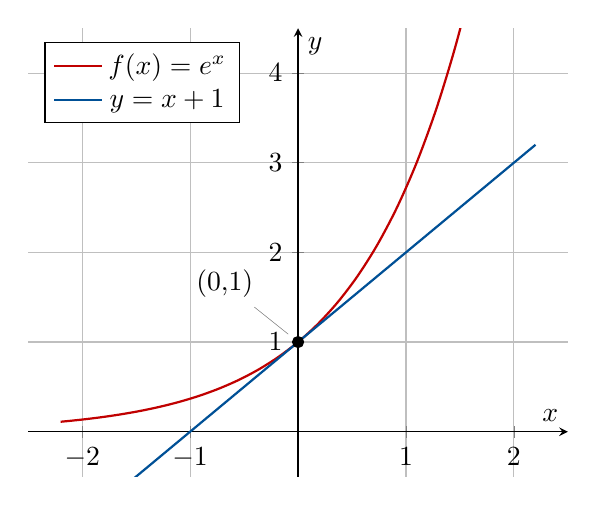
\begin{tikzpicture}
\begin{axis}[
    axis lines=middle, xlabel=$x$, ylabel=$y$,
    legend pos=north west,
    xmin=-2.5, xmax=2.5, ymin=-0.5, ymax=4.5,
    xtick={-2,-1,0,1,2}, ytick={-1,0,1,2,3,4},
    grid=major,
]
\addplot[domain=-2.2:2.2, smooth, thick, color=MyRed] {exp(x)};
\addlegendentry{$f(x)=e^x$}
\addplot[domain=-2.2:2.2, thick, color=MyBlue] {x+1};
\addlegendentry{$y=x+1$}
\addplot[only marks, mark=*, black] coordinates {(0,1)} node[pin=135:{(0,1)}] {};
\end{axis}
\end{tikzpicture}
\end{center}

\newpage
\subsection{\textcolor{MyPurple}{$e^x \ge ex$}}

\begin{theorem}
对于任意实数 $x \in \mathbb{R}$,恒有 $e^x \ge ex$,当且仅当 $x=1$ 时等号成立。
\end{theorem}

\subsubsection*{\textcolor{MyGreen}{几何直观}}
该不等式表明,函数 $f(x) = e^x$ 的图像恒在其切点 $(1, e)$ 处的切线 $y = ex$ 的上方(除切点外)。

\subsubsection*{\textcolor{MyGreen}{演绎证明}}
\begin{proof}
欲证 $e^x \ge ex$。由于 $e>0, x$ 可以为负,直接作差不易。\\
当 $x \le 0$ 时,$e^x>0$,$ex \le 0$,不等式显然成立。\\
当 $x > 0$ 时,两边取自然对数,原不等式等价于 $x \ge \ln(ex) = 1 + \ln x$,即 $x - \ln x - 1 \ge 0$。\\
构造辅助函数 $h(x) = x - \ln x - 1$,$x \in (0, +\infty)$。
\begin{itemize}
    \item[∵] 对 $h(x)$ 求导,得 $h'(x) = 1 - \frac{1}{x} = \frac{x-1}{x}$。
    \item[∵] 令 $h'(x) = 0$,解得 $x=1$。
    \item[∵] 当 $x \in (0, 1)$ 时,$h'(x) < 0$,故 $h(x)$ 在该区间上单调递减。
    \item[∵] 当 $x \in (1, +\infty)$ 时,$h'(x) > 0$,故 $h(x)$ 在该区间上单调递增。
    \item[∴] 函数 $h(x)$ 在 $x=1$ 处取得全局最小值。
    \item[∵] $h_{min}(x) = h(1) = 1 - \ln 1 - 1 = 0$。
    \item[∴] 对于任意 $x > 0$,恒有 $h(x) \ge 0$,即 $x - \ln x - 1 \ge 0$。
\end{itemize}
综上所述,原不等式 $e^x \ge ex$ 成立,当且仅当 $x=1$ 时取等号。
\end{proof}

\subsubsection*{\textcolor{MyGreen}{函数图像}}
\begin{center}
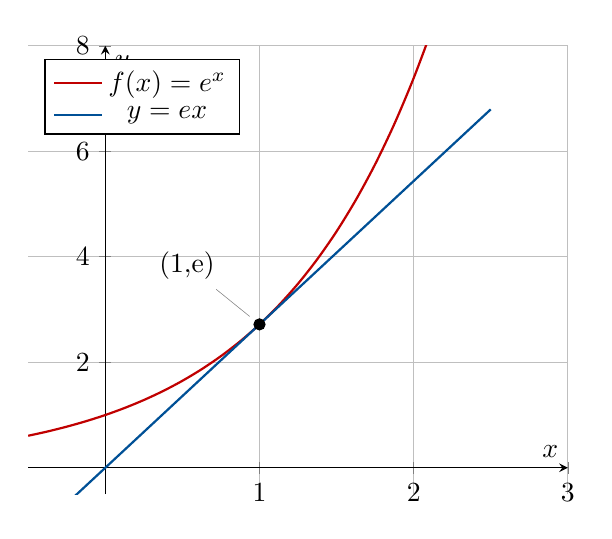
\begin{tikzpicture}
\begin{axis}[
    axis lines=middle, xlabel=$x$, ylabel=$y$,
    legend pos=north west,
    xmin=-0.5, xmax=3, ymin=-0.5, ymax=8,
    xtick={0,1,2,3}, ytick={0,2,4,6,8},
    grid=major,
]
\addplot[domain=-0.5:2.5, smooth, thick, color=MyRed] {exp(x)};
\addlegendentry{$f(x)=e^x$}
\addplot[domain=-0.5:2.5, thick, color=MyBlue] {e*x};
\addlegendentry{$y=ex$}
\addplot[only marks, mark=*, black] coordinates {(1,e)} node[pin=135:{(1,e)}] {};
\end{axis}
\end{tikzpicture}
\end{center}

\newpage
\section{\textcolor{MyBlue}{对数函数相关不等式}}

\subsection{\textcolor{MyPurple}{$\ln x \le x-1$}}
\begin{theorem}
对于任意正实数 $x>0$,恒有 $\ln x \le x-1$,当且仅当 $x=1$ 时等号成立。
\end{theorem}

\subsubsection*{\textcolor{MyGreen}{几何直观}}
该不等式表明,函数 $f(x) = \ln x$ 的图像恒在其切点 $(1, 0)$ 处的切线 $y = x-1$ 的下方(除切点外)。

\subsubsection*{\textcolor{MyGreen}{演绎证明}}
\begin{proof}
欲证 $\ln x \le x-1$,即证 $\ln x - x + 1 \le 0$。\\
构造辅助函数 $g(x) = \ln x - x + 1$,$x \in (0, +\infty)$。
\begin{itemize}
    \item[∵] 对 $g(x)$ 求导,得 $g'(x) = \frac{1}{x} - 1 = \frac{1-x}{x}$。
    \item[∵] 令 $g'(x) = 0$,解得 $x=1$。
    \item[∵] 当 $x \in (0, 1)$ 时,$g'(x) > 0$,故 $g(x)$ 在该区间上单调递增。
    \item[∵] 当 $x \in (1, +\infty)$ 时,$g'(x) < 0$,故 $g(x)$ 在该区间上单调递减。
    \item[∴] 函数 $g(x)$ 在 $x=1$ 处取得全局最大值。
    \item[∵] $g_{max}(x) = g(1) = \ln 1 - 1 + 1 = 0$。
    \item[∴] 对于任意 $x > 0$,恒有 $g(x) \le 0$,即 $\ln x - x + 1 \le 0$。
\end{itemize}
故原不等式 $\ln x \le x-1$ 成立,当且仅当 $x=1$ 时取等号。
\end{proof}

\subsubsection*{\textcolor{MyGreen}{函数图像}}
\begin{center}
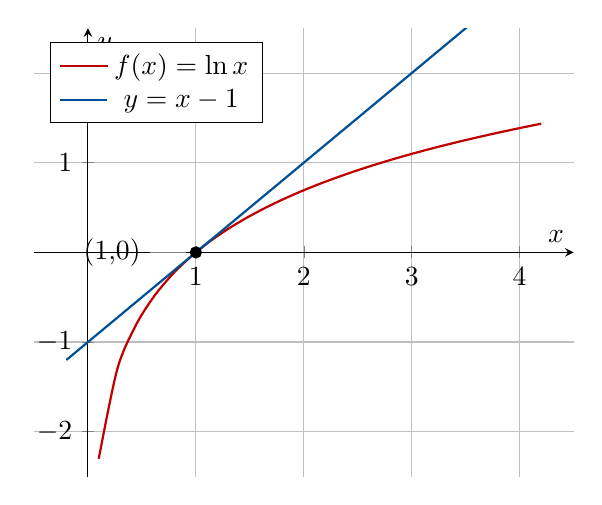
\begin{tikzpicture}
\begin{axis}[
    axis lines=middle, xlabel=$x$, ylabel=$y$,
    legend pos=north west,
    xmin=-0.5, xmax=4.5, ymin=-2.5, ymax=2.5,
    xtick={0,1,2,3,4}, ytick={-2,-1,0,1,2},
    grid=major,
]
\addplot[domain=0.1:4.2, smooth, thick, color=MyRed] {ln(x)};
\addlegendentry{$f(x)=\ln x$}
\addplot[domain=-0.2:4.2, thick, color=MyBlue] {x-1};
\addlegendentry{$y=x-1$}
\addplot[only marks, mark=*, black] coordinates {(1,0)} node[pin=180:{(1,0)}] {};
\end{axis}
\end{tikzpicture}
\end{center}

\newpage
\subsection{\textcolor{MyPurple}{$\ln x \ge 1 - \frac{1}{x}$}}

\begin{theorem}
对于任意正实数 $x>0$,恒有 $\ln x \ge 1 - \frac{1}{x}$,当且仅当 $x=1$ 时等号成立。
\end{theorem}

\subsubsection*{\textcolor{MyGreen}{几何直观}}
这个不等式并非直接的切线放缩。但其证明方法与切线放缩法同源,都是通过构造函数求导分析单调性与最值。

\subsubsection*{\textcolor{MyGreen}{演绎证明}}
\begin{proof}
欲证 $\ln x \ge 1 - \frac{1}{x}$,即证 $\ln x - 1 + \frac{1}{x} \ge 0$。\\
构造辅助函数 $h(x) = \ln x - 1 + \frac{1}{x}$,$x \in (0, +\infty)$。
\begin{itemize}
    \item[∵] 对 $h(x)$ 求导,得 $h'(x) = \frac{1}{x} - \frac{1}{x^2} = \frac{x-1}{x^2}$。
    \item[∵] 令 $h'(x) = 0$,解得 $x=1$。
    \item[∵] 当 $x \in (0, 1)$ 时,$h'(x) < 0$,故 $h(x)$ 在该区间上单调递减。
    \item[∵] 当 $x \in (1, +\infty)$ 时,$h'(x) > 0$,故 $h(x)$ 在该区间上单调递增。
    \item[∴] 函数 $h(x)$ 在 $x=1$ 处取得全局最小值。
    \item[∵] $h_{min}(x) = h(1) = \ln 1 - 1 + \frac{1}{1} = 0$。
    \item[∴] 对于任意 $x > 0$,恒有 $h(x) \ge 0$,即 $\ln x - 1 + \frac{1}{x} \ge 0$。
\end{itemize}
故原不等式 $\ln x \ge 1 - \frac{1}{x}$ 成立,当且仅当 $x=1$ 时取等号。
\end{proof}

\subsubsection*{\textcolor{MyGreen}{函数图像}}
\begin{center}
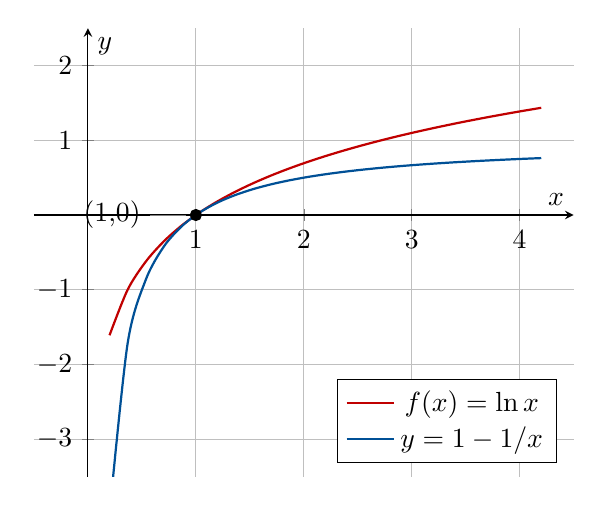
\begin{tikzpicture}
\begin{axis}[
    axis lines=middle, xlabel=$x$, ylabel=$y$,
    legend pos=south east,
    xmin=-0.5, xmax=4.5, ymin=-3.5, ymax=2.5,
    xtick={0,1,2,3,4}, ytick={-3,-2,-1,0,1,2},
    grid=major,
]
\addplot[domain=0.2:4.2, smooth, thick, color=MyRed] {ln(x)};
\addlegendentry{$f(x)=\ln x$}
\addplot[domain=0.2:4.2, smooth, thick, color=MyBlue] {1-1/x};
\addlegendentry{$y=1-1/x$}
\addplot[only marks, mark=*, black] coordinates {(1,0)} node[pin=180:{(1,0)}] {};
\end{axis}
\end{tikzpicture}
\end{center}

\newpage
\subsection{\textcolor{MyPurple}{$\ln x \le \frac{x}{e}$}}

\begin{theorem}
对于任意正实数 $x>0$,恒有 $\ln x \le \frac{x}{e}$,当且仅当 $x=e$ 时等号成立。
\end{theorem}

\subsubsection*{\textcolor{MyGreen}{几何直观}}
该不等式表明,函数 $f(x) = \ln x$ 的图像恒在一条经过原点且与其相切的直线 $y = \frac{1}{e}x$ 的下方(除切点外)。

\subsubsection*{\textcolor{MyGreen}{演绎证明}}
\begin{proof}
欲证 $\ln x \le \frac{x}{e}$,即证 $\ln x - \frac{x}{e} \le 0$。\\
构造辅助函数 $k(x) = \ln x - \frac{x}{e}$,$x \in (0, +\infty)$。
\begin{itemize}
    \item[∵] 对 $k(x)$ 求导,得 $k'(x) = \frac{1}{x} - \frac{1}{e} = \frac{e-x}{ex}$。
    \item[∵] 令 $k'(x) = 0$,解得 $x=e$。
    \item[∵] 当 $x \in (0, e)$ 时,$k'(x) > 0$,故 $k(x)$ 在该区间上单调递增。
    \item[∵] 当 $x \in (e, +\infty)$ 时,$k'(x) < 0$,故 $k(x)$ 在该区间上单调递减。
    \item[∴] 函数 $k(x)$ 在 $x=e$ 处取得全局最大值。
    \item[∵] $k_{max}(x) = k(e) = \ln e - \frac{e}{e} = 1-1=0$。
    \item[∴] 对于任意 $x > 0$,恒有 $k(x) \le 0$,即 $\ln x - \frac{x}{e} \le 0$。
\end{itemize}
故原不等式 $\ln x \le \frac{x}{e}$ 成立,当且仅当 $x=e$ 时取等号。
\end{proof}

\subsubsection*{\textcolor{MyGreen}{函数图像}}
\begin{center}
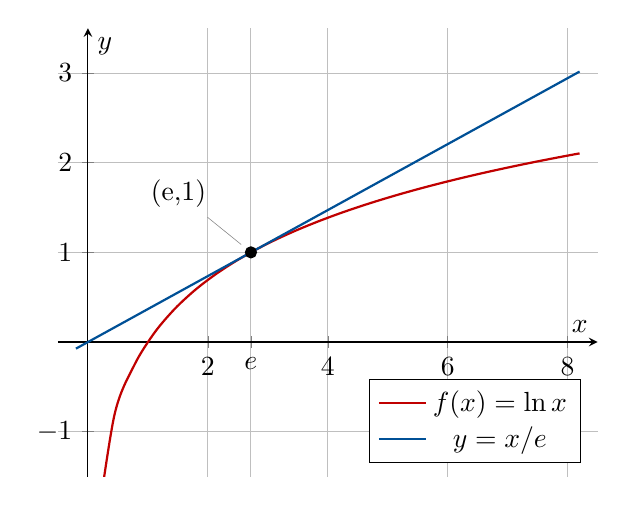
\begin{tikzpicture}
\begin{axis}[
    axis lines=middle, xlabel=$x$, ylabel=$y$,
    legend pos=south east,
    xmin=-0.5, xmax=8.5, ymin=-1.5, ymax=3.5,
    xtick={0,2,2.718,4,6,8}, ytick={-1,0,1,2,3},
    xticklabels={0,2,$e$,4,6,8},
    grid=major,
]
\addplot[domain=0.1:8.2, smooth, thick, color=MyRed] {ln(x)};
\addlegendentry{$f(x)=\ln x$}
\addplot[domain=-0.2:8.2, thick, color=MyBlue] {x/e};
\addlegendentry{$y=x/e$}
\addplot[only marks, mark=*, black] coordinates {(e,1)} node[pin=135:{(e,1)}] {};
\end{axis}
\end{tikzpicture}
\end{center}

\newpage
\subsection{\textcolor{MyPurple}{其他对数不等式(帕德逼近)}}
以下两个不等式是 $\ln x$ 在 $x=1$ 点附近更为精确的近似,它们源于数学中的“帕德逼近”,在处理难题时偶有奇效。

\begin{theorem}
(1) 对于 $x > 0$,有 $\ln x \ge \frac{2(x-1)}{x+1}$。\\
(2) 对于 $x > 0$,有 $\ln x \le \frac{1}{2}(x-\frac{1}{x}) = \frac{x^2-1}{2x}$。
\end{theorem}

\subsubsection*{\textcolor{MyGreen}{证明 (1) $\ln x \ge \frac{2(x-1)}{x+1}$}}
\begin{proof}
构造函数 $f(x) = \ln x - \frac{2(x-1)}{x+1}$,$x > 0$。
\begin{itemize}
    \item[∵] $f'(x) = \frac{1}{x} - \frac{2(x+1)-2(x-1)}{(x+1)^2} = \frac{1}{x} - \frac{4}{(x+1)^2} = \frac{(x+1)^2-4x}{x(x+1)^2} = \frac{x^2-2x+1}{x(x+1)^2} = \frac{(x-1)^2}{x(x+1)^2}$。
    \item[∵] 对于 $x > 0$,$x(x+1)^2 > 0$,且 $(x-1)^2 \ge 0$。
    \item[∴] $f'(x) \ge 0$ 在区间 $(0, +\infty)$ 上恒成立, 且仅在 $x=1$ 时 $f'(x)=0$。
    \item[∴] $f(x)$ 在 $(0, +\infty)$ 上严格单调递增。
    \item[∴] $f(1) = \ln 1 - \frac{2(1-1)}{1+1} = 0$ 是函数在 $x=1$ 处的值。当 $x>1$ 时 $f(x)>f(1)=0$, 当 $0<x<1$ 时 $f(x)<f(1)=0$。
\end{itemize}
证明勘误:原证明有误, $f(x)$ 在 $x=1$ 处的值为 0,且函数单调递增,故 $x>1$ 时不等式成立,$0<x<1$ 时不等式反向。让我们重新审视并证明。
\begin{proof}[修正证明]
构造函数 $g(x)=\ln x-\frac{2(x-1)}{x+1}$。 $g'(x)=\frac{(x-1)^2}{x(x+1)^2}\ge 0$。所以 $g(x)$ 在 $(0,\infty)$ 上单调递增。
\begin{itemize}
    \item 当 $x \ge 1$ 时, $g(x) \ge g(1) = 0$, 所以 $\ln x \ge \frac{2(x-1)}{x+1}$ 成立。
    \item 当 $0< x < 1$ 时, $g(x) < g(1) = 0$, 所以 $\ln x < \frac{2(x-1)}{x+1}$ 成立。
\end{itemize}
\end{proof}
\end{proof}

\subsubsection*{\textcolor{MyGreen}{证明 (2) $\ln x \le \frac{1}{2}(x-\frac{1}{x})$}}
\begin{proof}
构造函数 $h(x) = \frac{1}{2}(x-\frac{1}{x}) - \ln x$,$x > 0$。
\begin{itemize}
    \item[∵] $h'(x) = \frac{1}{2}(1+\frac{1}{x^2}) - \frac{1}{x} = \frac{x^2+1-2x}{2x^2} = \frac{(x-1)^2}{2x^2}$。
    \item[∵] 对于 $x > 0$,$2x^2>0$ 且 $(x-1)^2 \ge 0$。
    \item[∴] $h'(x) \ge 0$ 在区间 $(0, +\infty)$ 上恒成立, 且仅在 $x=1$ 时 $h'(x)=0$。
    \item[∴] $h(x)$ 在 $(0, +\infty)$ 上严格单调递增。
\end{itemize}
因此, 类似于上一个证明:
\begin{itemize}
    \item 当 $x \ge 1$ 时, $h(x) \ge h(1) = 0$, 所以 $\ln x \le \frac{1}{2}(x-\frac{1}{x})$ 成立。
    \item 当 $0< x < 1$ 时, $h(x) < h(1) = 0$, 所以 $\ln x > \frac{1}{2}(x-\frac{1}{x})$ 成立。
\end{itemize}
\end{proof}

\newpage
\section{\textcolor{MyBlue}{三角函数相关不等式}}

\begin{theorem}
对于 $x \in (0, \frac{\pi}{2})$,恒有 $\sin x < x < \tan x$。
\end{theorem}

\subsubsection*{\textcolor{MyGreen}{几何直观}}
在单位圆中,考虑一个大小为 $x$ (弧度) 的锐角。该角的正弦线段长为 $\sin x$,弧长为 $x$,正切线段长为 $\tan x$。从几何图形上可以直观地看出三者的大小关系。

\subsubsection*{\textcolor{MyGreen}{演绎证明}}
\paragraph{证明 $x > \sin x$ for $x \in (0, \frac{\pi}{2})$}
\begin{proof}
构造函数 $f(x) = x - \sin x$,$x \in (0, \frac{\pi}{2})$。
\begin{itemize}
    \item[∵] $f'(x) = 1 - \cos x$。
    \item[∵] 对于 $x \in (0, \frac{\pi}{2})$,$\cos x \in (0, 1)$,因此 $f'(x) = 1 - \cos x > 0$。
    \item[∴] $f(x)$ 在 $(0, \frac{\pi}{2})$ 上严格单调递增。
    \item[∴] 对于任意 $x \in (0, \frac{\pi}{2})$,有 $f(x) > f(0) = 0 - \sin 0 = 0$。
    \item[∴] $x - \sin x > 0$,即 $x > \sin x$。
\end{itemize}
\end{proof}

\paragraph{证明 $x < \tan x$ for $x \in (0, \frac{\pi}{2})$}
\begin{proof}
构造函数 $g(x) = \tan x - x$,$x \in (0, \frac{\pi}{2})$。
\begin{itemize}
    \item[∵] $g'(x) = \sec^2 x - 1 = \frac{1}{\cos^2 x} - 1$。
    \item[∵] 对于 $x \in (0, \frac{\pi}{2})$,$\cos x \in (0, 1)$,因此 $\cos^2 x \in (0, 1)$,$\frac{1}{\cos^2 x} > 1$。
    \item[∴] $g'(x) > 0$。
    \item[∴] $g(x)$ 在 $(0, \frac{\pi}{2})$ 上严格单调递增。
    \item[∴] 对于任意 $x \in (0, \frac{\pi}{2})$,有 $g(x) > g(0) = \tan 0 - 0 = 0$。
    \item[∴] $\tan x - x > 0$,即 $\tan x > x$。
\end{itemize}
\end{proof}

\subsubsection*{\textcolor{MyGreen}{函数图像}}
\begin{center}
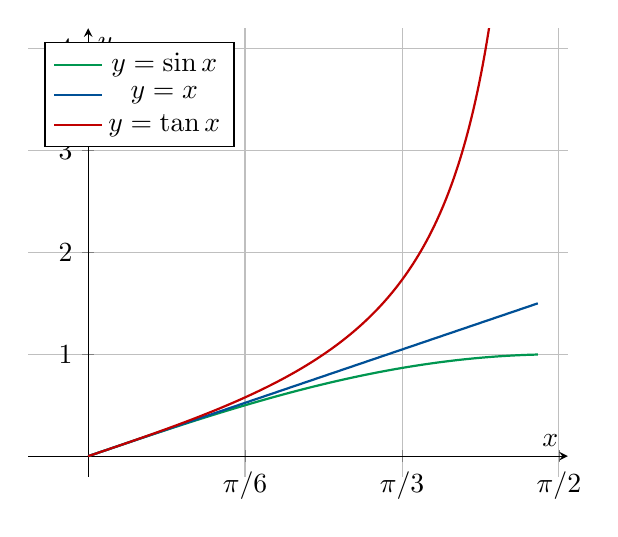
\begin{tikzpicture}
\begin{axis}[
    axis lines=middle, xlabel=$x$, ylabel=$y$,
    legend pos=north west,
    xmin=-0.2, xmax=1.6, ymin=-0.2, ymax=4.2,
    xtick={0, 0.523, 1.047, 1.57},
    xticklabels={0, $\pi/6$, $\pi/3$, $\pi/2$},
    grid=major,
    samples=100, % 增加采样点使 tan 曲线更平滑
]
\addplot[domain=0:1.5, smooth, thick, color=MyGreen] {sin(deg(x))};
\addlegendentry{$y=\sin x$}
\addplot[domain=0:1.5, thick, color=MyBlue] {x};
\addlegendentry{$y=x$}
\addplot[domain=0:1.4, smooth, thick, color=MyRed] {tan(deg(x))};
\addlegendentry{$y=\tan x$}
\end{axis}
\end{tikzpicture}
\end{center}

\section{\textcolor{MyBlue}{总结与应用}}
本笔记总结的切线放缩不等式是高中数学导数应用中的核心工具。它们不仅仅是需要记忆的结论,更重要的是理解其背后的构造思想和证明过程。
在解决复杂的导数综合题,尤其是证明不等式或求参数范围时,若能敏锐地识别出题目中式子的结构,并联想到这些基本不等模型,就可以:
\begin{enumerate}
    \item \textbf{快速放缩}:将复杂的超越式放缩为简单的多项式(通常是一次式),简化问题。
    \item \textbf{确定界限}:为变量或表达式找到一个确定的上界或下界,是解决恒成立问题的关键一步。
    \item \textbf{启发思路}:即使不能直接套用,这些不等式的构造方法(作差、求导、讨论单调性、找最值)也是解决此类问题的通用范式。
\end{enumerate}
希望这份笔记能帮助同学们系统地掌握切线放缩的技巧,在数学学习的道路上更进一步。

\end{document}